\documentclass{NRVposter}
\usepackage{graphicx}
\usepackage{hyperref}
\usepackage{wrapfig}

\title{NRV Framework}
\author{T. Couppey\textsuperscript{2}, L. Regnacq\textsuperscript{1, 2}, R. Giraud\textsuperscript{1, 2}, O. Romain\textsuperscript{2}, Y. Bornat\textsuperscript{1}, F. Kolbl\textsuperscript{1, 2}}
\institute{
    \textsuperscript{1} Laboratory IMS - UMR CNRS 5218, Bordeaux INP, U. Bordeaux - Talence, France\\
    \textsuperscript{2} Laboratory ETIS - UMR CNRS 8051, CYU, ENSEA - Cergy, France}
\begin{document}
\maketitle

% Tip: for long titles, use \parbox{\linewidth}{text}

%\block{Abstract}{This is a description of the class to make posters according 
%to NRV's official template.}

\begin{columns}
\column{0.62}
\block{The NeuRon Virtualizer: a pythonic tool for simulating neural interfaces}{
    NRV is a pythonic framework to enable fast and user-friendly simulations of the Peripheral Nervous System. Axons models are simulated with the NEURON software, and extracellular fields are computed either from analytic equations such as point source approximation or with a more detailed description of the nerve and electrode geometry and Finite Elements Method, either using COMSOL (additional commercial licence required) or the FENICS project. Stimulation waveform can be of random shapes, and any kinds of electrode can be combined to model complex stimulation strategies.

    \vspace{
        0.01\textheight
    }

    NRV has been optimized for large population of axons, from generating realistic population following a specific diameter probability, through automatic placement to computation and post-processing of the axons' activity when a stimulus is applied. Parallel computation, interface with NEURON and COMSOL and FENICS is automatically handled by NRV. A complete documentation is also available for detailed description and full help on installation, basic usage and API reference.
    \vspace{
        0.01\textheight
    }
    \begin{center}
        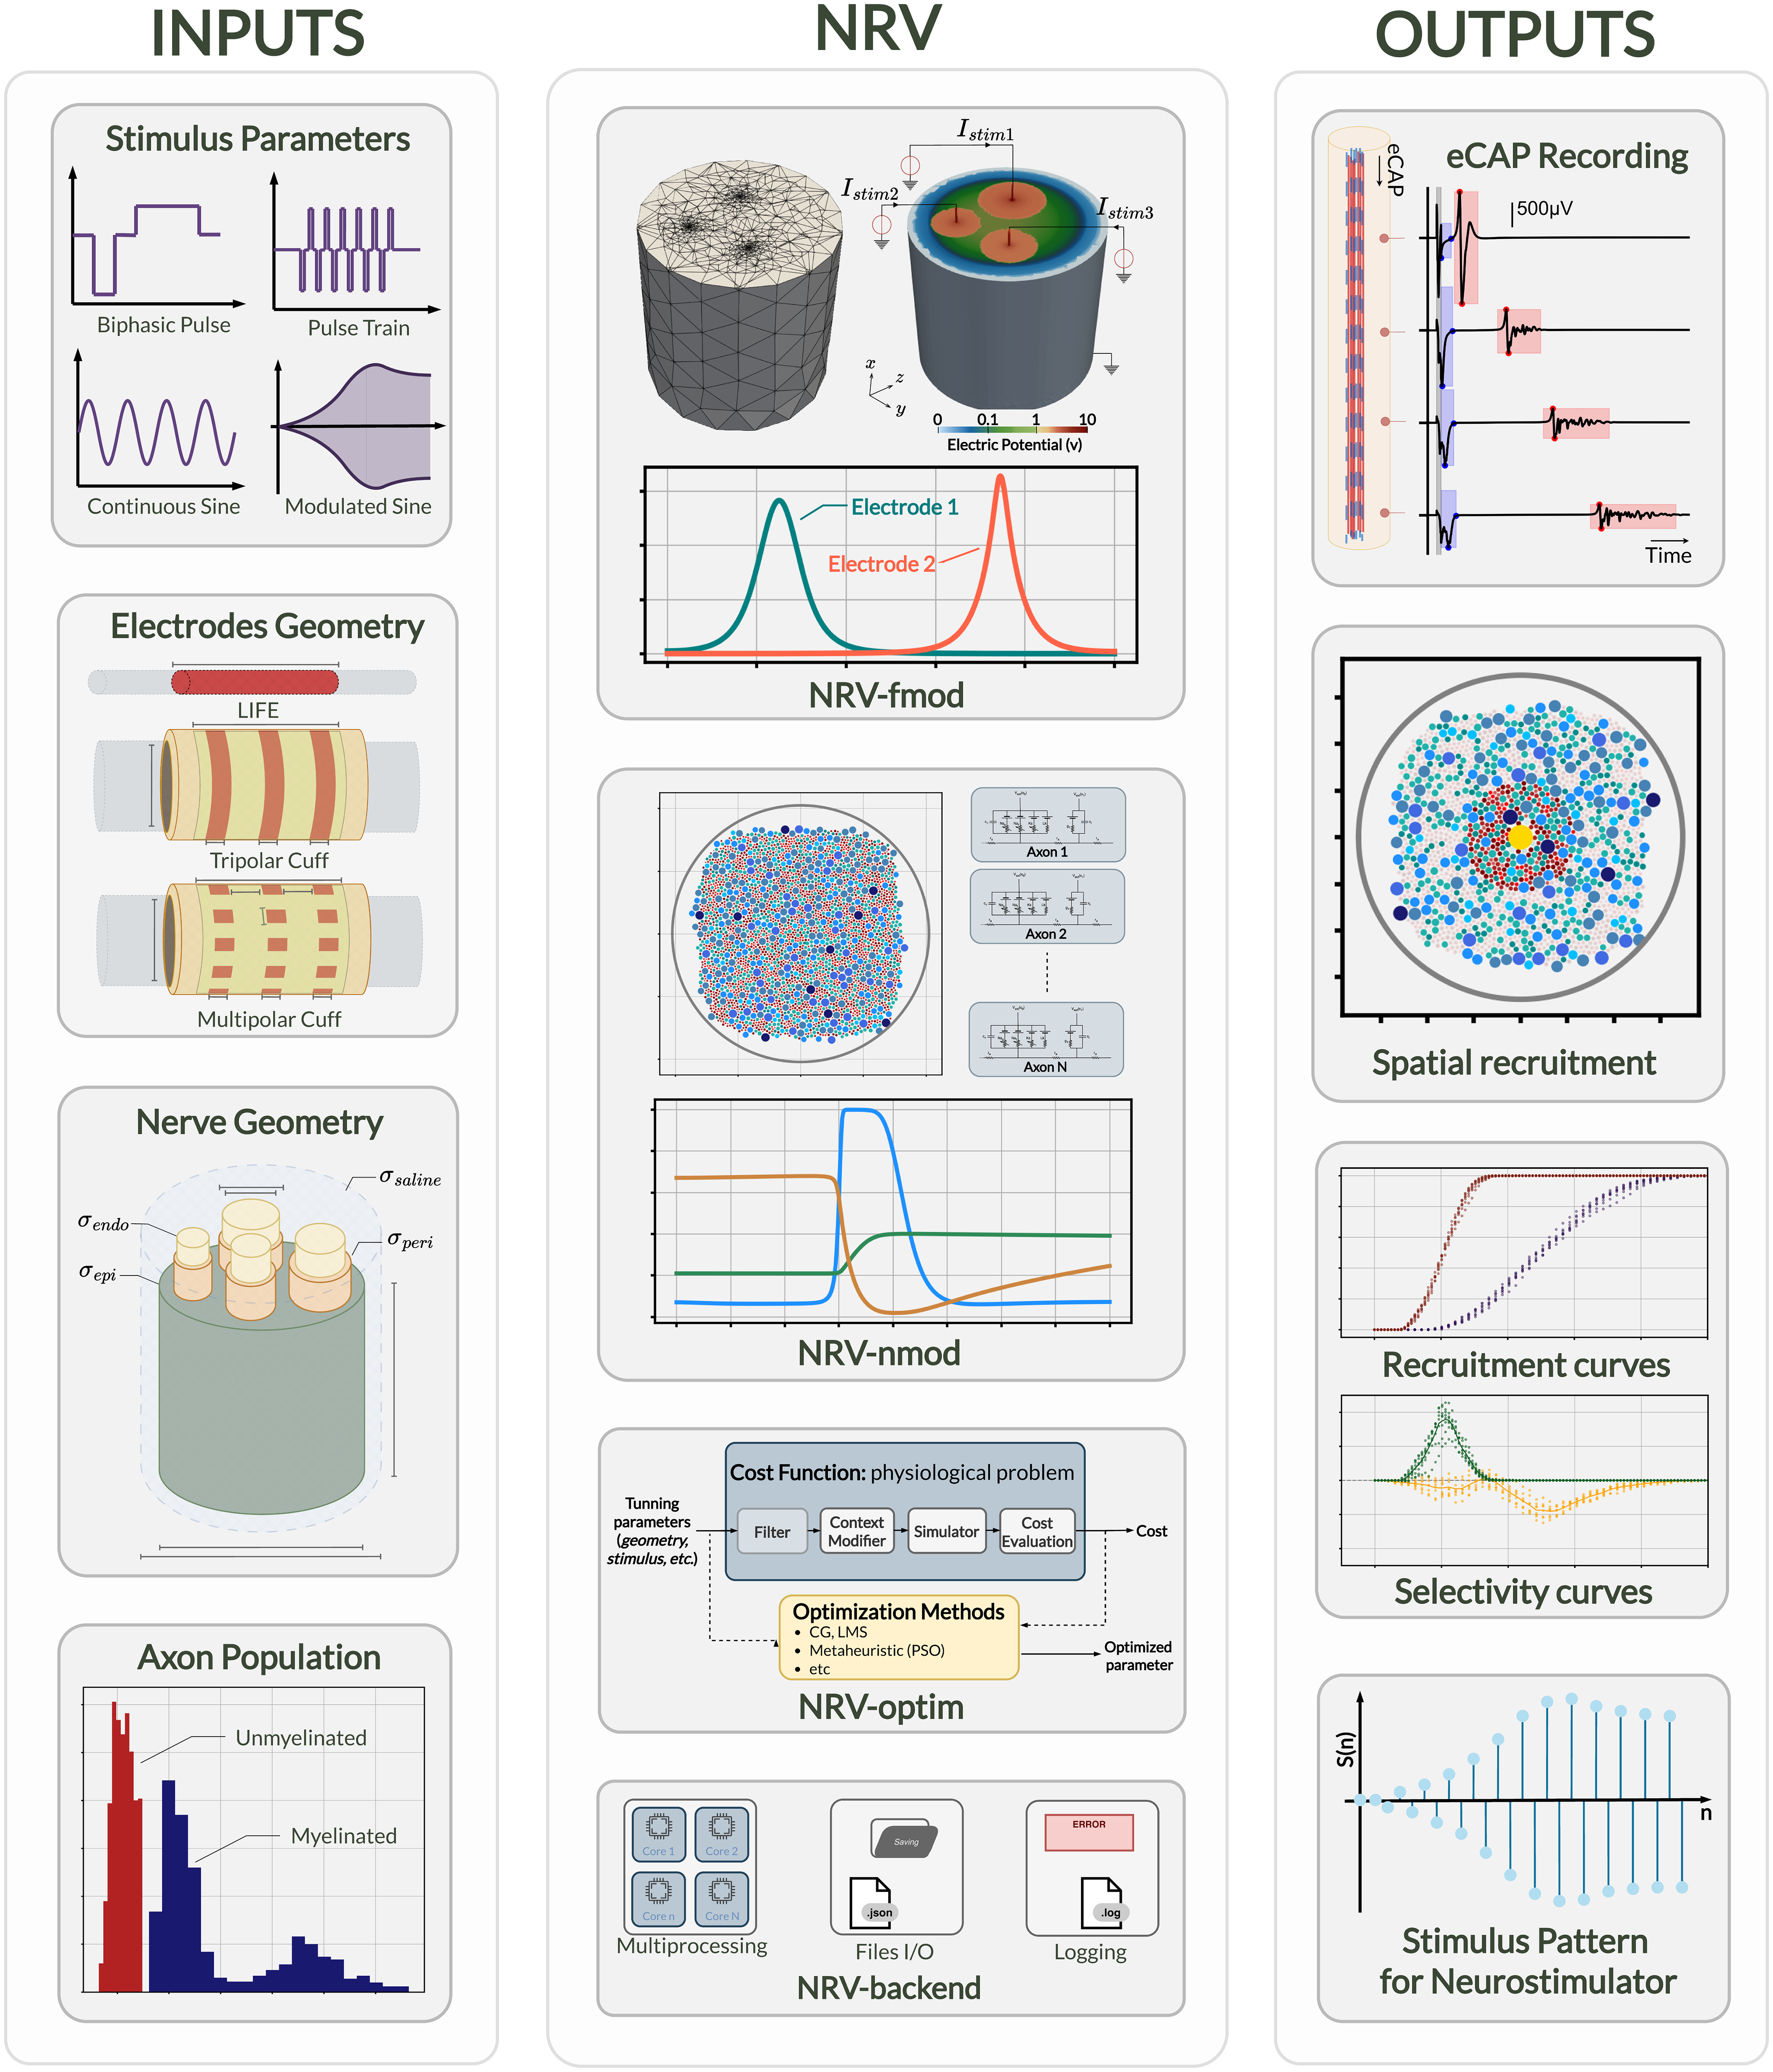
\includegraphics[width=0.45\columnwidth]{./images/overview.png}
    \end{center}
    \vspace{
        0.01\textheight
    }
    It also allows the simulation of complex strategies such as multiple electrode combinations and waveforms ranging from conventional biphasic pulses to more complex modulated kHz stimuli. In addition, we provide automated support for stimulation strategy optimization and handle the computational backend transparently to the user. Our framework has been extensively tested and validated with several existing results in the literature.
}

\block{Dependencies - Open source approach}{

NRV is free and open source (under CeCILL 2.1 license). Dependencies are also open source projects:
\begin{itemize}
    \item NEURON (\url{https://neuron.yale.edu/neuron/}),
    \item FEniCSX (\url{https://fenicsproject.org}),
    \item GMSH (\url{https://gmsh.info}).
\end{itemize}
COMSOL is used as an optional dependency (for comparison purpose only).\\
\vspace{0.01\textheight}
}

 

\column{0.38}
\block{Find us}
{
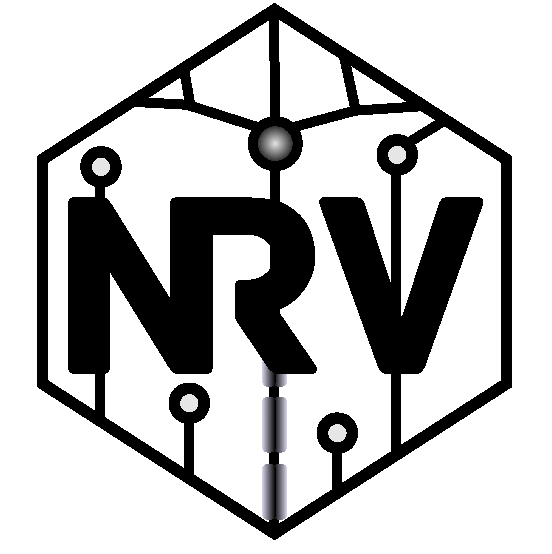
\includegraphics[width=0.015\columnwidth]{./images/NRV_bw.pdf}  \textbf{Access our website:} \\ \url{https://nrv-framework.org}\\
            \begin{center}
                
\includegraphics[width=0.08\columnwidth]{./images/qrcode_website.png}
            \end{center}
            and enter the forum for help (community page)\\

\includegraphics[width=0.015\columnwidth]{./images/github_logo.png} \textbf{Access the source code:} \\ \url{https://github.com/nrv-framework/NRV}\\
            \begin{center}
                
\includegraphics[width=0.08\columnwidth]{./images/qrcode_github.png}
            \end{center}

\includegraphics[width=0.015\columnwidth]{./images/pypi_logo.png} \textbf{Get the installer:} \\ \url{https://pypi.org/project/nrv-py/}\\
        \begin{center}
            
\includegraphics[width=0.08\columnwidth]{./images/qrcode_pypi.png}
        \end{center}

\includegraphics[width=0.015\columnwidth]{./images/rtd_logo.png} \textbf{Get the documentation:} \\ \url{https://nrv.readthedocs.io/en/latest/}\\
        \begin{center}
            
\includegraphics[width=0.08\columnwidth]{./images/qrcode_rtd.png}
        \end{center}

}

\block{Scientific foundations - How to cite}{

    \begin{center}
        
\includegraphics[width=0.08\columnwidth]{./images/qrcode_PLOSpaper.png} 
    \end{center}
    Couppey, T., Regnacq, L., Giraud, R., Romain, O., Bornat, Y., $\&$ Kolbl, F. (2024). NRV: An open framework for in silico evaluation of peripheral nerve electrical stimulation strategies. PLOS Computational Biology, 20(7), e1011826.
}

\block{Contribute}{
    NRV is designed for the community in neuroscience and biomedical engineering. If you want to join, use, develop feel free to fork. Contact us at:\\
    \url{contact@nrv-framework.org}\\
    or meet us on the forum at:\\
    \url{nrv-framework.org/forum}
    \begin{center}
        
\includegraphics[width=0.08\columnwidth]{./images/qrcode_forum.png}
    \end{center}

}

\end{columns}


\end{document}

